\section{Related works}
\label{sec:releated_works}

\textbf{Open-Vocabulary Feature Distillation.}
Recent works have embedded 2D vision-language features into 3D scene representations to enable open-vocabulary 3D understanding. Pioneering efforts on NeRFs such as LERF~\cite{kerr2023lerf} and OpenNeRF~\cite{engelmann2024opennerf} used CLIP~\cite{radford2021clip} embeddings and pixel-aligned features, enabling open-vocabulary queries.
However, due to the computational needs of NeRF~\cite{mildenhall2020nerf}, they face scalability and efficiency bottlenecks. Thus, subsequent works have embedded language features into 3DGS~\cite{zuo2024fmgs, shi2024language, zhou2024feature}. LangSplat~\cite{qin2024langsplat} employs SAM~\cite{kirillov2023sam} to extract multi-level CLIP features, then compresses dimensionality with an autoencoder to build a compact yet expressive 3D language field. Feature3DGS~\cite{zhou2024feature} uses a convolutional neural network (CNN) to lift feature dimensions. Although both approaches aim to compress the supervision signal, this dimensionality reduction inevitably results in information loss. GOI~\cite{goi2024} and CCL-LGS~\cite{tian2025ccl} employ a single trainable feature codebook to store language embeddings, with an MLP predicting discrete codebook indices for rasterized 2D feature maps, which compress semantics spatially rather than dimensionally and retain semantic richness. However, as these approaches rely on 2D rendered feature maps for perception, their performance in 3D scene understanding is significantly limited. 

Other methods first group 3D Gaussians or points into semantically meaningful clusters, typically corresponding to objects or parts, and then assign a language feature to each cluster as a whole~\cite{liang2024supergseg, wu2024opengaussian, goi2024, li2024instancegaussian, piekenbrinck2025opensplat3d, jiang2025votesplat}. These methods introduce an explicit discrete grouping step as a form of prior semantic structuring: OpenGaussian~\cite{wu2024opengaussian} performs coarse-to-fine clustering based on spatial proximity followed by feature similarity. SuperGSeg~\cite{liang2024supergseg} and InstanceGaussian~\cite{li2024instancegaussian} both leverage neural Gaussians to model instance-level features: SuperGSeg groups Gaussians into Super-Gaussians to facilitate language assignment, whereas InstanceGaussian directly assigns fused semantic features to each cluster. VoteSplat~\cite{jiang2025votesplat} and OpenSplat3D~\cite{piekenbrinck2025opensplat3d} mitigate the pixel-level ambiguities of the direct distillation. Then, the resulting cluster graph structures support higher-level reasoning~\cite{liang2024supergseg, zhan2025hi}, which per-Gaussian features cannot easily enable. However, all these methods rely on feature distillation using per-cluster learnable language embeddings. These approaches are computationally expensive and highly sensitive to noise or outliers in the preprocessed feature maps, since the language features are optimized directly in Euclidean space. As a result, even minor errors in the input features can propagate through the model, leading to inconsistent or inaccurate semantic representations, particularly in complex or cluttered scenes.

\begin{figure*}[t]
    \centering
    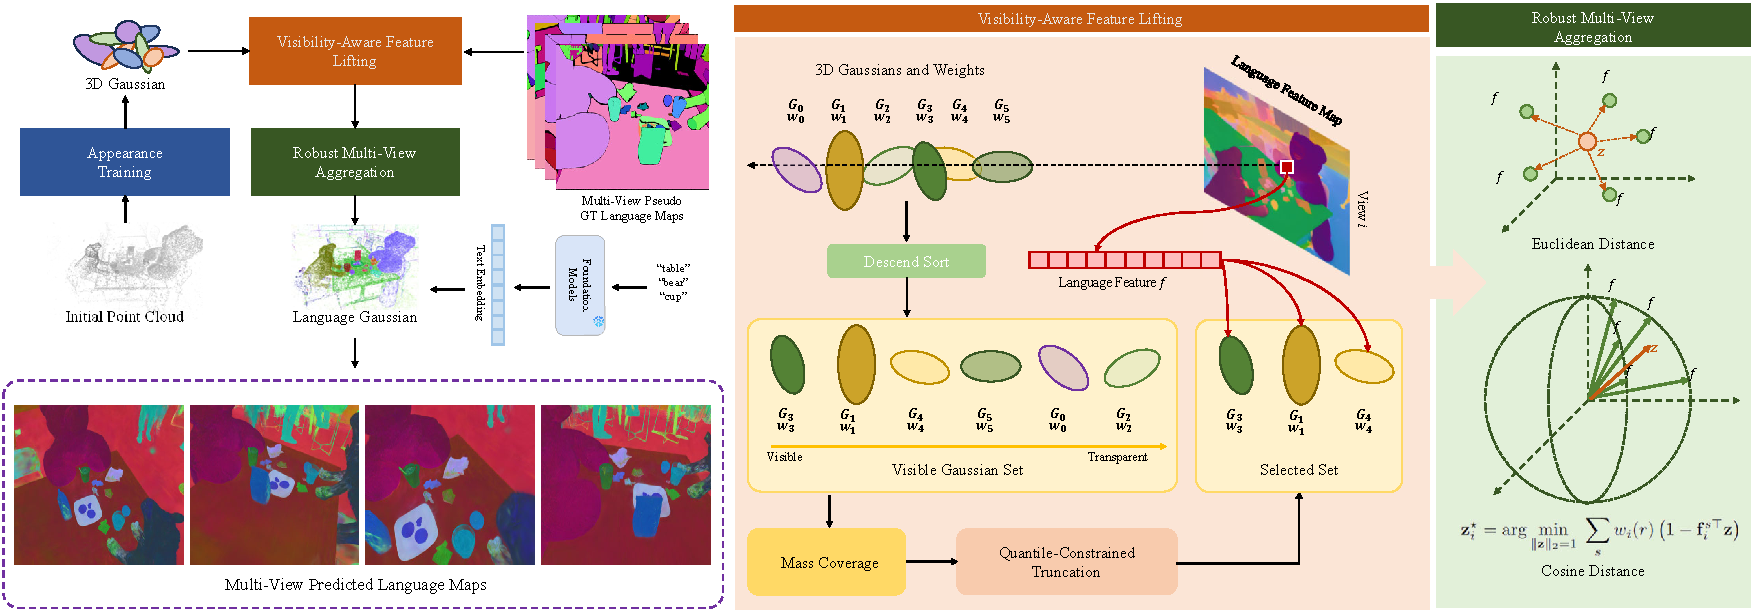
\includegraphics[width=\linewidth]{figs/main_methods.pdf}
    \vspace{-5mm}
    \caption{Overview of VALA. The framework is shown on the left, with the orange and green blocks detailed on the right being our key contributions: the visibility-aware feature lifting (orange, Section~\ref{sec:gating}), and the robust multi-view aggregation (green, Section~\ref{sec:median}).}
    \label{fig:main_method}
    \vspace{-5mm}
\end{figure*}

\textbf{Open-Vocabulary Feature Aggregation.}
Beyond cluster-based language features distillation, recent works adopt more efficient strategies for feature aggregation. For instance, Dr.Splat~\cite{drsplat25} and Occam's LGS~\cite{cheng2024occam} bypass intermediate 2D supervision and clustering by directly injecting language features into 3D Gaussians, achieving fast, accurate results in a training-free regime. While these direct feature aggregation methods deliver strong runtime efficiency and segmentation accuracy, they indiscriminately propagate 2D features to \emph{every} Gaussian intersected by each camera ray, disregarding scene geometry and occlusion. As a result, features from foreground objects (e.g., a vase) are erroneously assigned to background elements (e.g., the table or floor). Moreover, existing methods share two critical limitations: (i) they assign equal supervision to all Gaussians along a ray, ignoring each Gaussian’s marginal contribution to the rendered pixel, and (ii) they overlook the view-dependent noise and inconsistency in 2D language features. We address these issues with VALA, a robust and efficient training-free framework that improves open-vocabulary grounding through visibility-aware gating (for contribution-aligned supervision) and robust multi-view aggregation.
